\documentclass[17pt]{extarticle}
\usepackage[T1]{fontenc}
\usepackage[utf8]{inputenc}

\usepackage{amsfonts, amsmath, amssymb}
\usepackage{mathtools}

\usepackage{geometry}
 \geometry{
 a4paper,
 landscape,
 left=10mm,
 right = 10mm,
 top=10mm,
 bottom=10mm,
 }

\usepackage{graphicx}
\usepackage{subfig}

\pagenumbering{gobble}
\usepackage{url}
%%  Defines the command \url{} that can be used to typeset url:s
%%  in text

\usepackage[parfill]{parskip}
\usepackage{ragged2e}
\usepackage{mathptmx}
\usepackage{anyfontsize}
\usepackage{t1enc}

\newcommand*{\pd}[2]{\ensuremath{\dfrac{\partial #1}{\partial #2}}}
\newcommand*{\inpd}[2]{\ensuremath{\frac{\partial #1}{\partial #2}}}
\DeclarePairedDelimiter\floor{\lfloor}{\rfloor}

\setcounter{tocdepth}{4}
\setcounter{secnumdepth}{4}

\begin{document}
\begin{center}
{\fontsize{200}{20}\selectfont Artificial}

\vfill

{\fontsize{200}{20}\selectfont Neural}

\vfill

{\fontsize{200}{20}\selectfont Networks}
\end{center}

\newpage
%%%%%%%%%%%%%%%%%%%%%%%%%%%%%%%%%%%%%%%%%%%%%%%%%%%%%%%%%%%%%%%%%%%%%%%%%%%%%%%%%%%%


\begin{center}
{\fontsize{60}{20}\selectfont Feed-forward Neural Networks}

\vfill

{\fontsize{60}{20}\selectfont Loss Function}

\vfill

{\fontsize{60}{20}\selectfont Gradient Descent}

\vfill

{\fontsize{60}{20}\selectfont Training Neural Networks}

\vfill

{\fontsize{60}{20}\selectfont Dense Face Detection}

\vfill

{\fontsize{60}{20}\selectfont Style Transfer}
\end{center}

\newpage
%%%%%%%%%%%%%%%%%%%%%%%%%%%%%%%%%%%%%%%%%%%%%%%%%%%%%%%%%%%%%%%%%%%%%%%%%%%%%%%%%%%%
\begin{center}
{\fontsize{40}{20}\selectfont Feed-forward Neural Networks}
\end{center}

Artificial neural networks are a machine learning model which draws inspiration from the biological brain. the model is constructed hierarchically as layers of neurons stack on top of each other. The first layer is given an input and is used to compute the value of the next layer. The layers are constructed sequentially such that the neurons at layer $l$ is the input to layer $l+1$. The process of propagating the given input through all the layers in neural network, up to the output layer, is called forward propagation. The most basic type of neural network is the feed-forward neural network. Every neuron in layer $l$ is connected to all the neurons in layer $l+1$. The network learns to predict accurate results by optimize the strength of the connections (called weights) between every pair of neurons.

\vfill
\begin{figure}[h]
	\centering %1.65
  		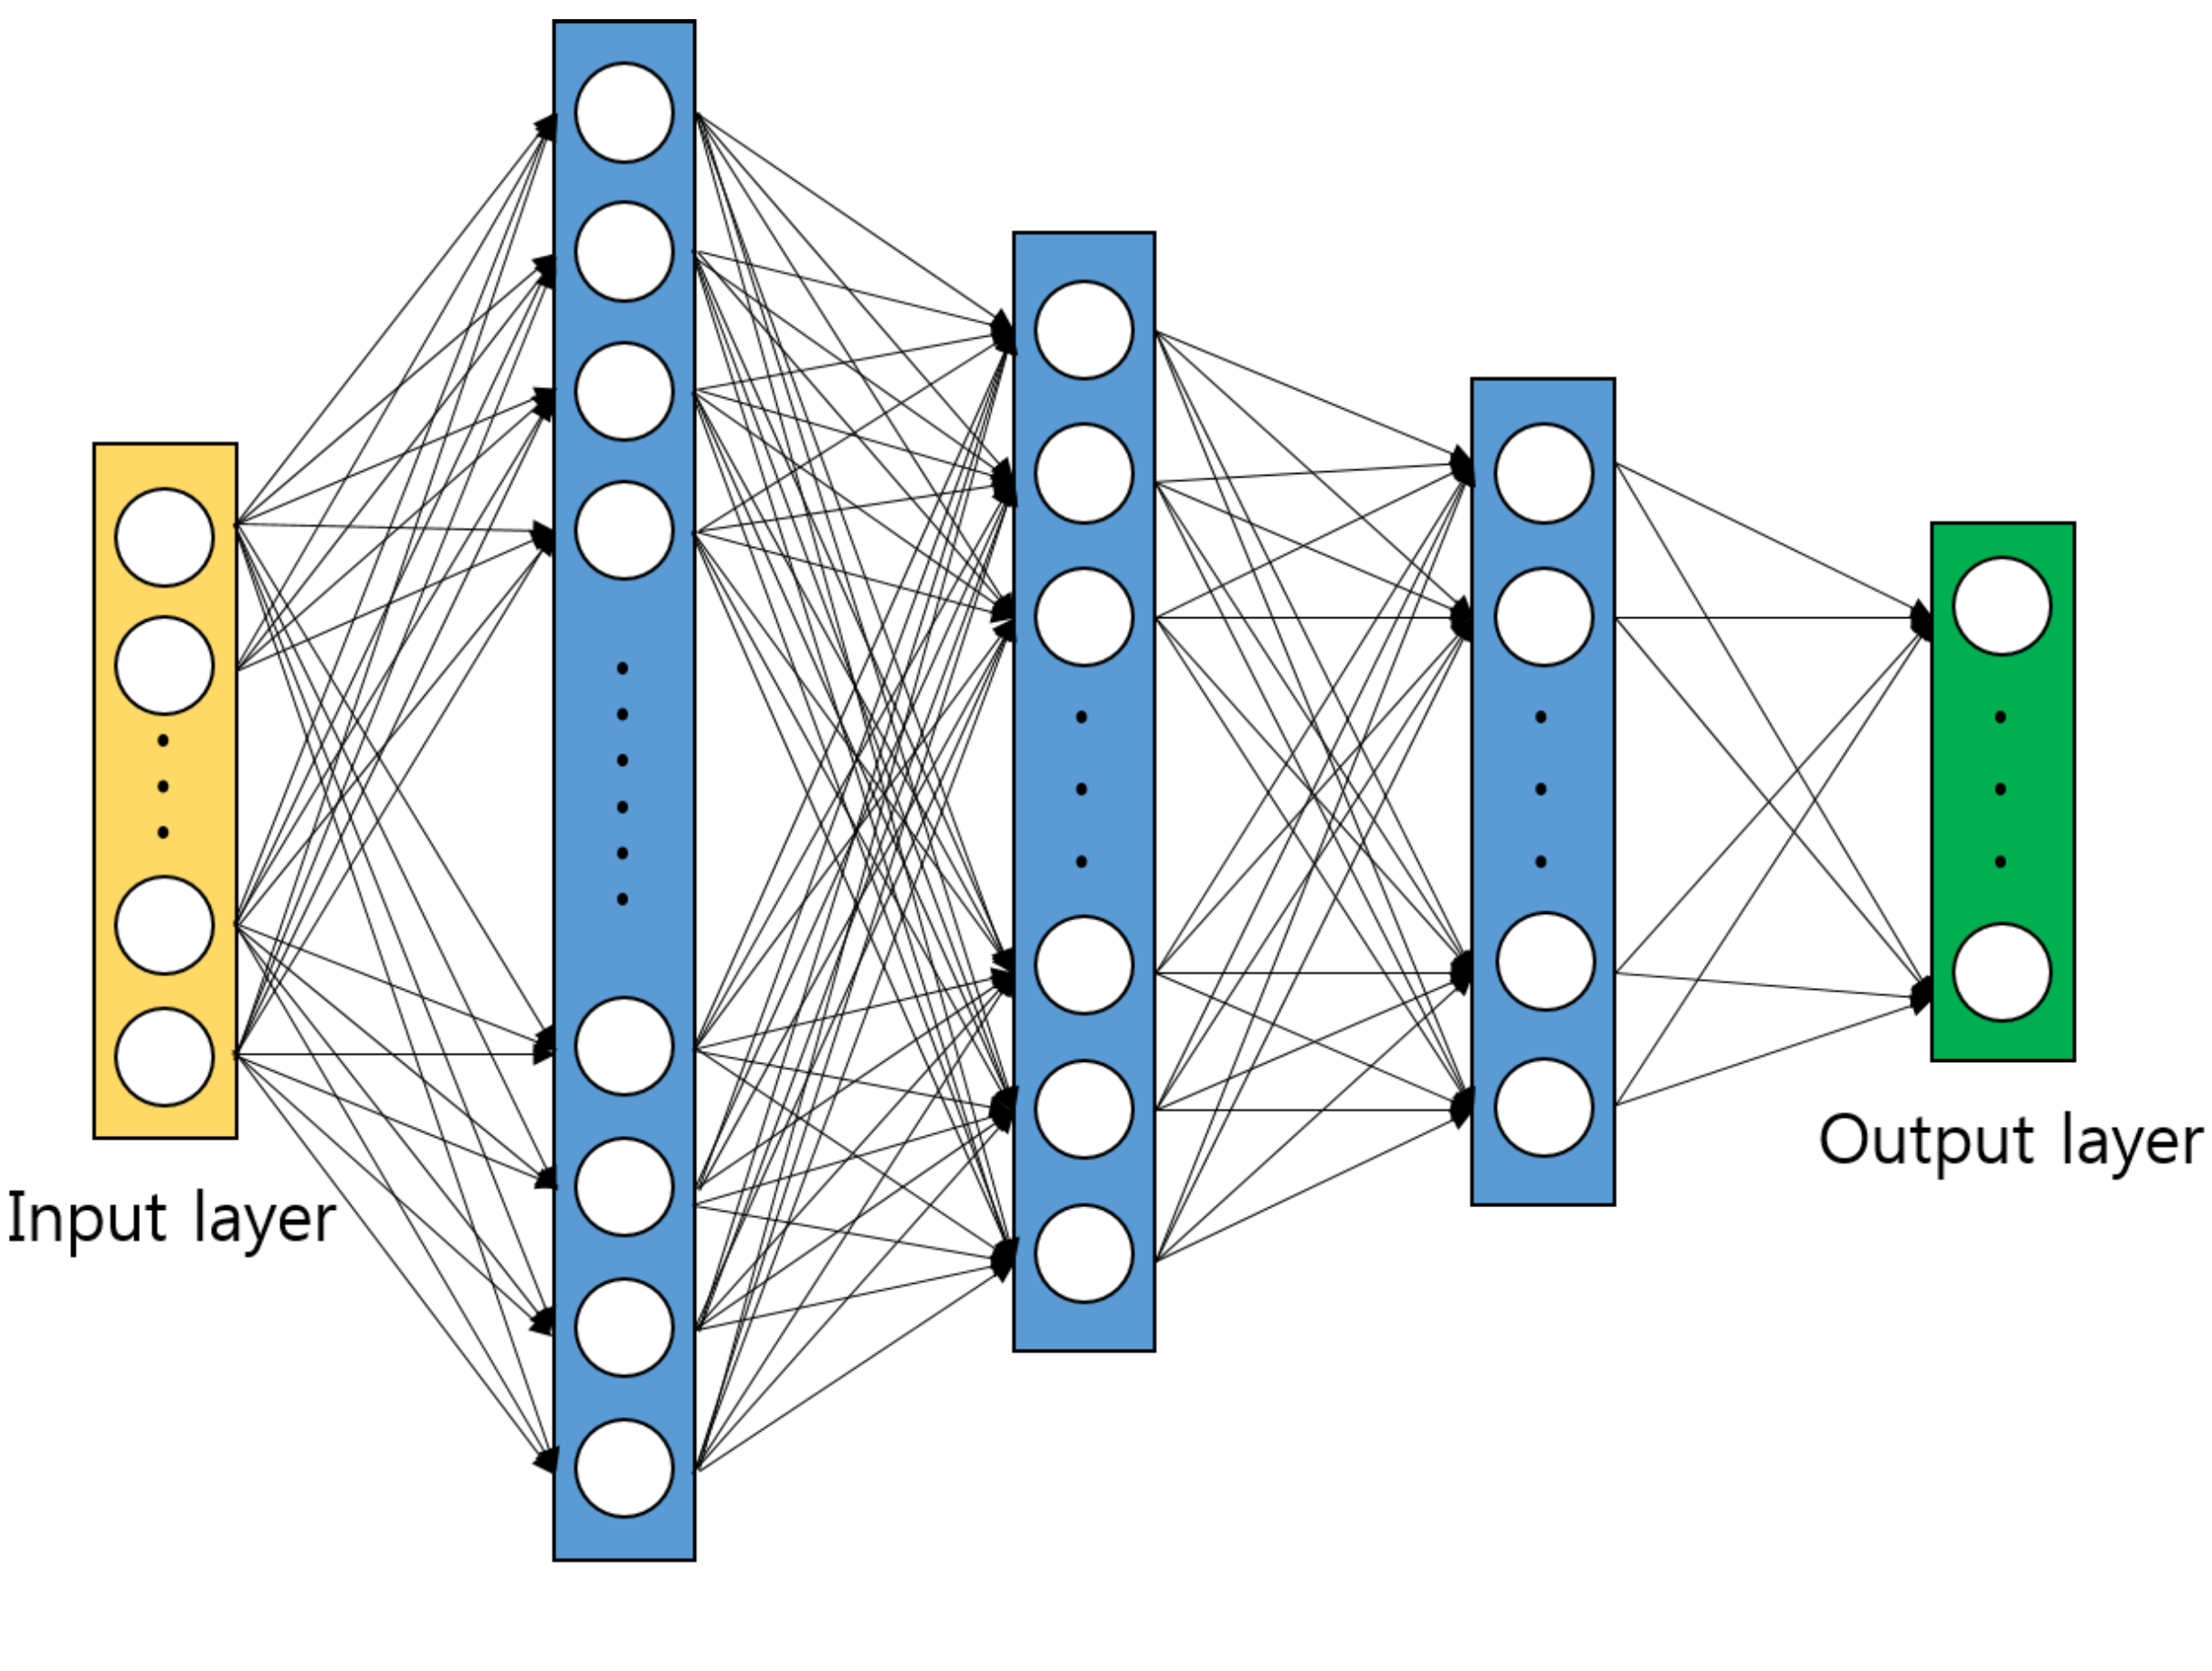
\includegraphics[scale=1.49]{entropy-19-00454-g002.png}
\end{figure}


\newpage
%%%%%%%%%%%%%%%%%%%%%%%%%%%%%%%%%%%%%%%%%%%%%%%%%%%%%%%%%%%%%%%%%%%%%%%%%%%%%%%%%%%%

The input is processed in batches of $R$. Let $N$ and $N'$ be the amount of neurons at layer $l$ and $l+1$ respectively. The neurons at layer $l$ can be expressed as a matrix $X^{(l)} \in \mathbb{R}^{R \times N}$. The weights between every pair of neurons are stored in a matrix $W^{(l)} \in \mathbb{R}^{N'}  \times N$ such that $W_{j, i}^{(l)}$ is the strength of the connection between neuron $X_{r, i}^{(l)}$ and $X_{r, j}^{(l+1)}$. Additionally, every layer $l$ has a bias neuron $b^{(l)} \in \mathbb{R}$ that is connected to every neuron in the next layer. Forward propagation can be express mathematically as:
\begin{align*}
Z^{(l+1)} & = X^{(l)}W^{(l)}+b^{(l)}\\
X^{(l+1)} & = f(Z^{(l+1)})
\end{align*}
Where $f$ is an element-wise non-linear function (usually ReLU, sigmoid or tanh).

Given an input $X$ and a human labeled ground truth $y$ the model wants to predict values $\hat{y}$ which resembles the ground truth as closely as possible. It is achieved by defining a multivariate loss function $L(\theta; X, y)$  with the network's parameters $\theta$ (all the weights and biases) with respect to a single training mini-batch $(X, y)$. The loss function describes the quality of the neural network's prediction $\hat{y}$ such that a lower loss represents a more accurate prediction. To simplify noration $L(\theta)$ is used to denote the loss function with respect to one mini-batch $(X, y)$ of training data. One way of defining the loss function is to use the mean squared error defined by the following equation:
\begin{equation}\label{MSE}
L(\theta) = \frac{1}{RN^{(L)}} \sum^{R}_{r=1} \sum^{N^{(L)}}_{i=1} (\hat{y}_{r,i}-y_{r,i})^2
\end{equation}
Here $R$ is the batch size and $N^{(L)}$ is the number of neurons in the last layer $L$.

The process of minimizing the loss function is called training. The model iterates through supervised training data and calculates the loss with respect to a mini-batch of training examples. Since the given input $X$ and ground truth $y$ stays fixed, the network learns by optimizing its weights $W^{(l)}$ and biases $b^{(l)}$ for every layer $l$ to decrease the loss.
\newpage
%%%%%%%%%%%%%%%%%%%%%%%%%%%%%%%%%%%%%%%%%%%%%%%%%%%%%%%%%%%%%%%%%%%%%%%%%%%%%%%%%%%%
\begin{center}
{\fontsize{40}{20}\selectfont Gradient Descent}
\end{center}


The gradient $\nabla L(\theta)$ is a vector of partial derivatives with respect to the parameters $\theta$ of the function $L$ and shows the direction of steepest ascent in the point ($\theta_{1}$, $\theta_{2}$, ..., $\theta_{n}$) in the $n$-dimensional vector space $\mathbb{R}^{n}$:
\begin{equation*}\label{EQgradientspace}
\nabla L(\theta) : \mathbb{R}^n \to \mathbb{R}^n
\end{equation*}
\begin{equation*}\label{EQgradientvector}
\nabla L(\theta) = 
	\begin{pmatrix} 
		\pd{L(\theta)}{\theta_{1}}, & 
		\pd{L(\theta)}{\theta_{2}}, &
		\cdots, &
		\pd{L(\theta)}{\theta_{n}}
		
		\end{pmatrix}
\end{equation*}

Gradient descent is the method of iteratively changing the values of the parameters $\theta$ proportionally to the negative gradient $-\nabla L(\theta)$ to minimize the function $L(\theta)$. The most basic algorithm of gradient descent is called Stochastic Gradient Descent (SGD) and uses the hyperparameter $\alpha$, called learning rate, to control the magnitude of the gradient. It is called Stochastic Gradient Descent because, at each iteration, the mini-batch responsible for the losses is randomly chosen and sampled from the whole batch of training data. SGD is defined by the following equations:

\begin{equation*}\label{EQgradient}
\pd{L(\theta)}{\theta_i} = \nabla_{\theta_i} L(\theta)
\end{equation*}
\begin{equation*}\label{SGD}
{\theta_i} \to {\theta_i} - \alpha \pd{L(\theta)}{\theta_i}
\end{equation*}
\begin{figure}[h]
  		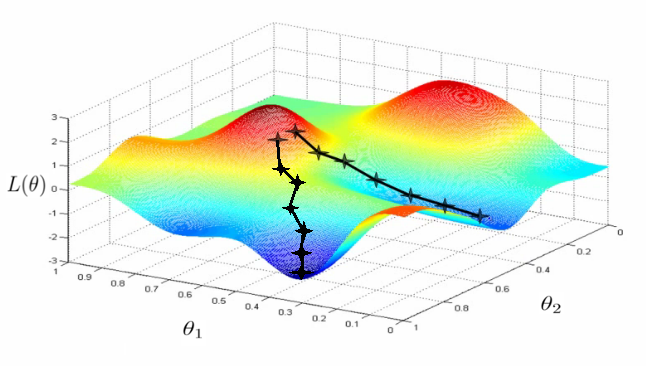
\includegraphics[scale=1.9]{gradient-descent.png}

{An illustration of Stochastic Gradient Descent on a function of two variables. Red regions symbolizes a high function value while blue regions symbolizes a low function value. The parameters were initialized near the global maximum and their values are altered iteratively to move in the direction of the negative gradient: the direction of steepest descent, to find a local minimum.}
\end{figure}

\newpage
%%%%%%%%%%%%%%%%%%%%%%%%%%%%%%%%%%%%%%%%%%%%%%%%%%%%%%%%%%%%%%%%%%%%%%%%%%%%%%%%%%%%

\begin{center}
{\fontsize{40}{20}\selectfont Training Neural Networks}
\end{center}

The neural network is trained by dividing the training data into mini-batches of size $R$. A mini-batch is then forward propagated and the loss is calculated with the loss function. The loss is then used in a process called backpropagation (explained in my paper) to propagate the models error through the network. The error is used to calculate the gradient by computing the partial derivative of the loss function with respect to the neural networks parameters (weights and biases). When the gradient has been fully computed one iteration of the gradient descent algorithm is applied to update the weights and biases of the neural network. This process is repeated until all the networks parameters have converged.
  	
  	
\newpage
%%%%%%%%%%%%%%%%%%%%%%%%%%%%%%%%%%%%%%%%%%%%%%%%%%%%%%%%%%%%%%%%%%%%%%%%%%%%%%%%%%%%
%FACE DETECTION


\begin{figure}[h]
  		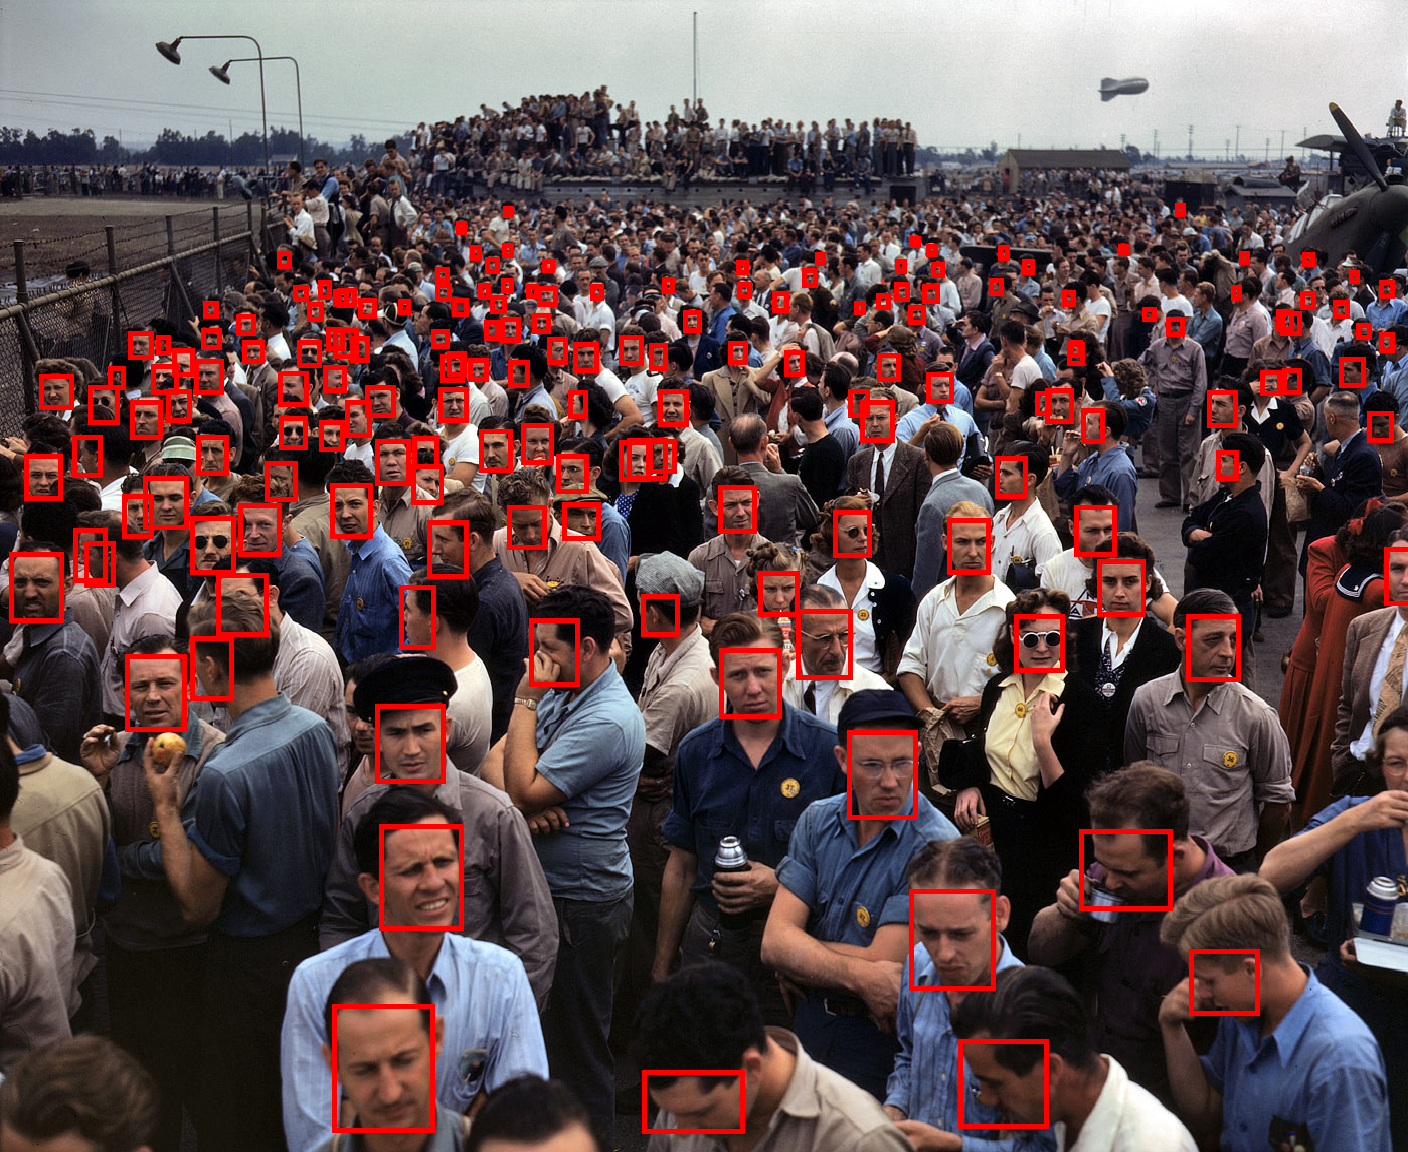
\includegraphics[scale=0.58]{resultscrowd.png}
\end{figure}

\begin{figure}[h]
  		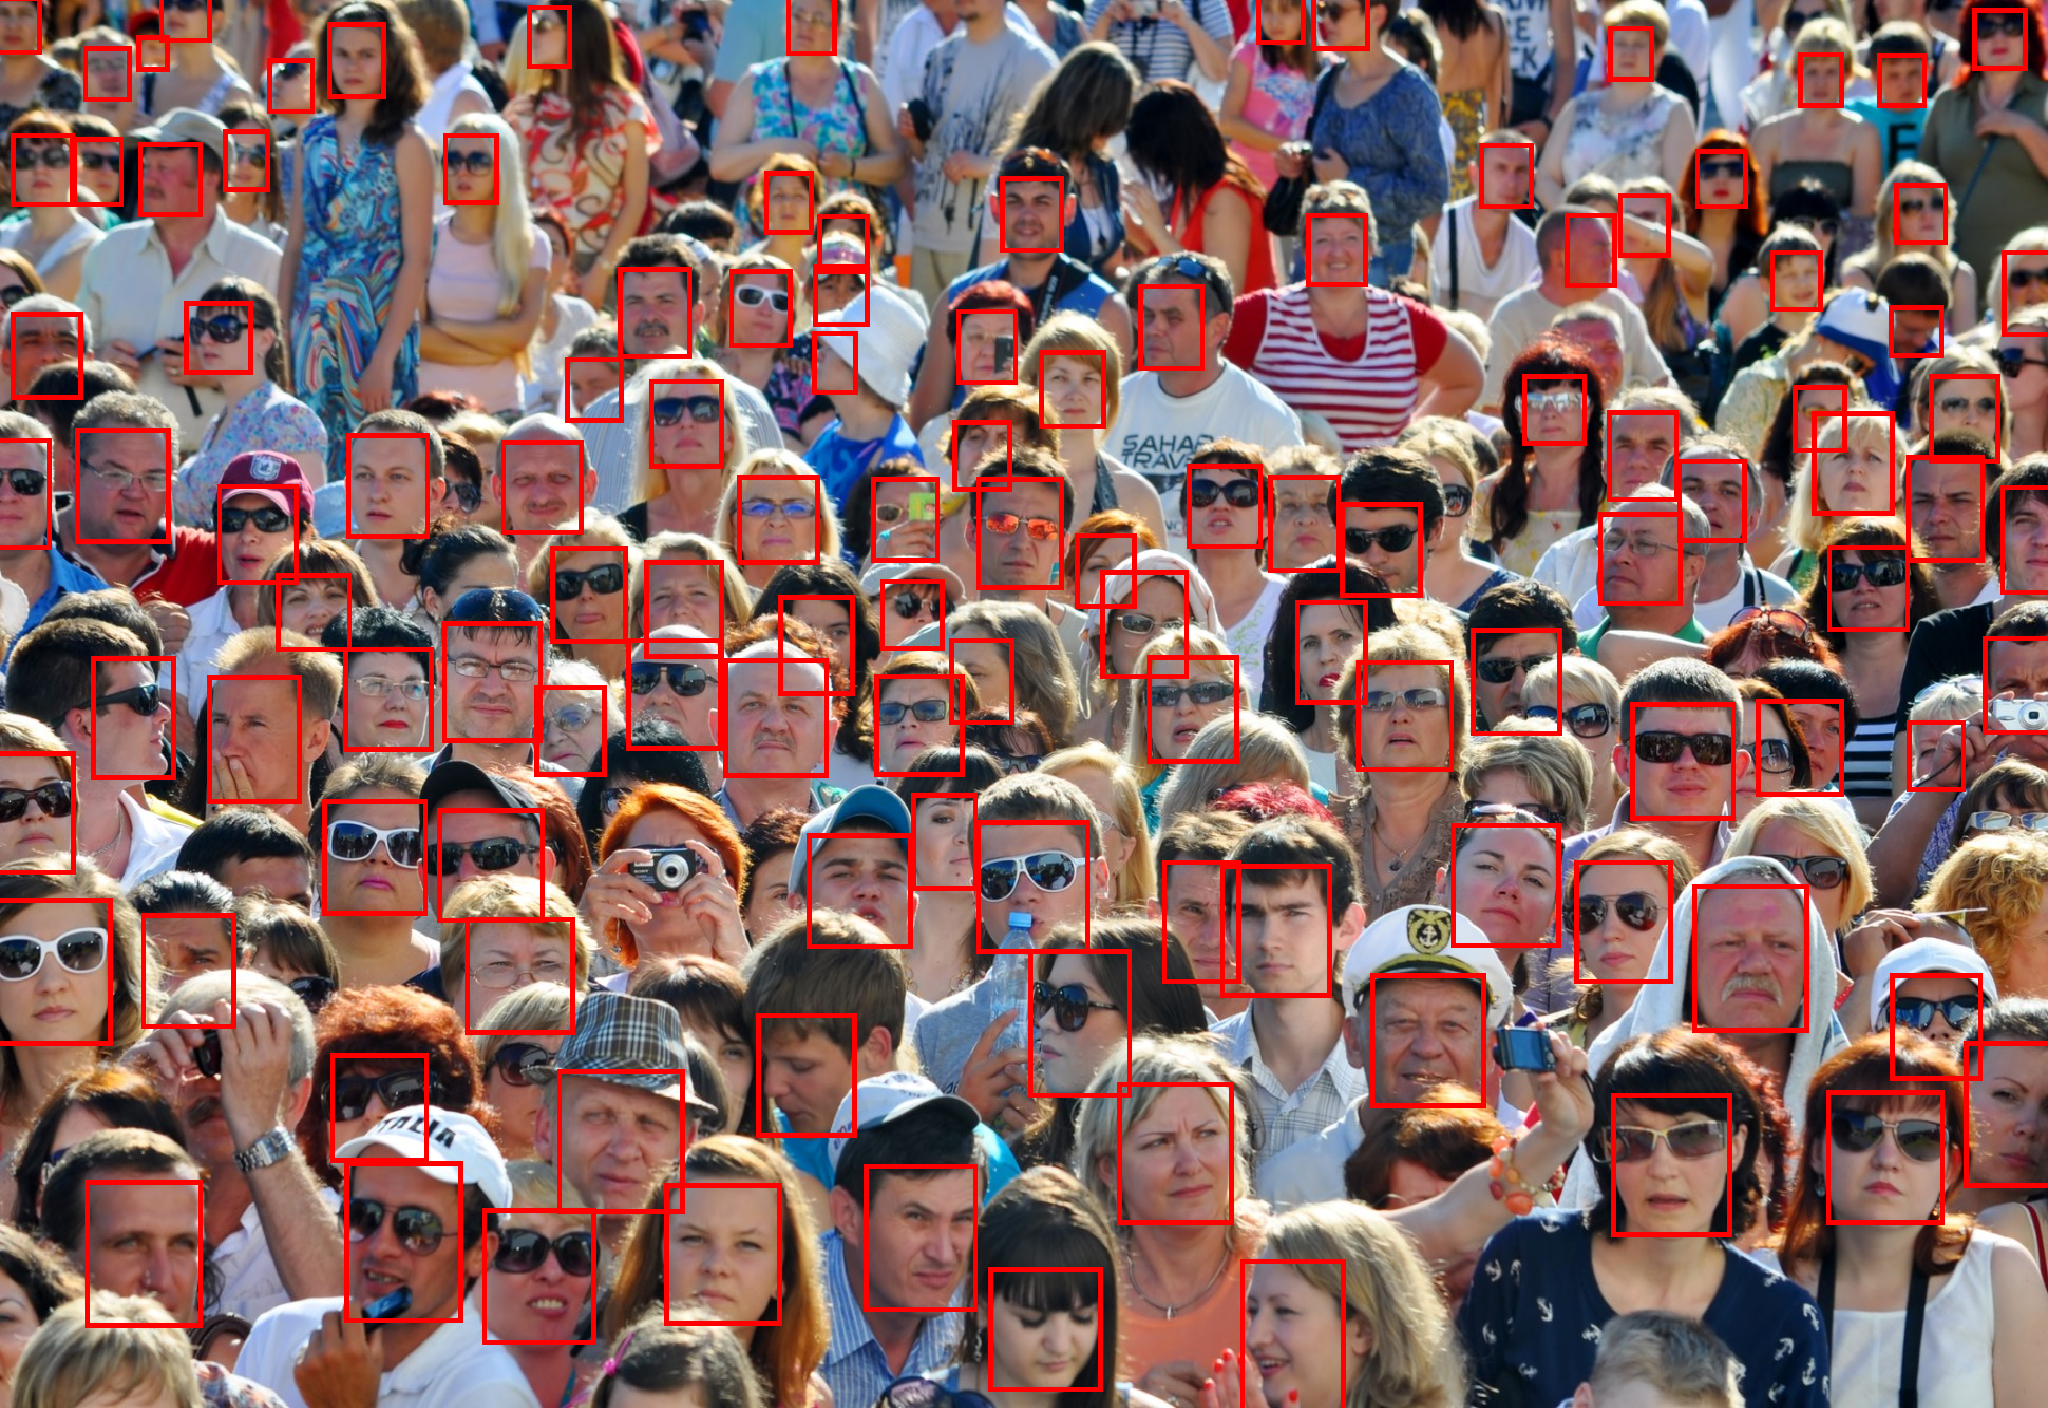
\includegraphics[scale=0.41]{resultscrowd2.png}
\end{figure}

\begin{figure}[h]
  		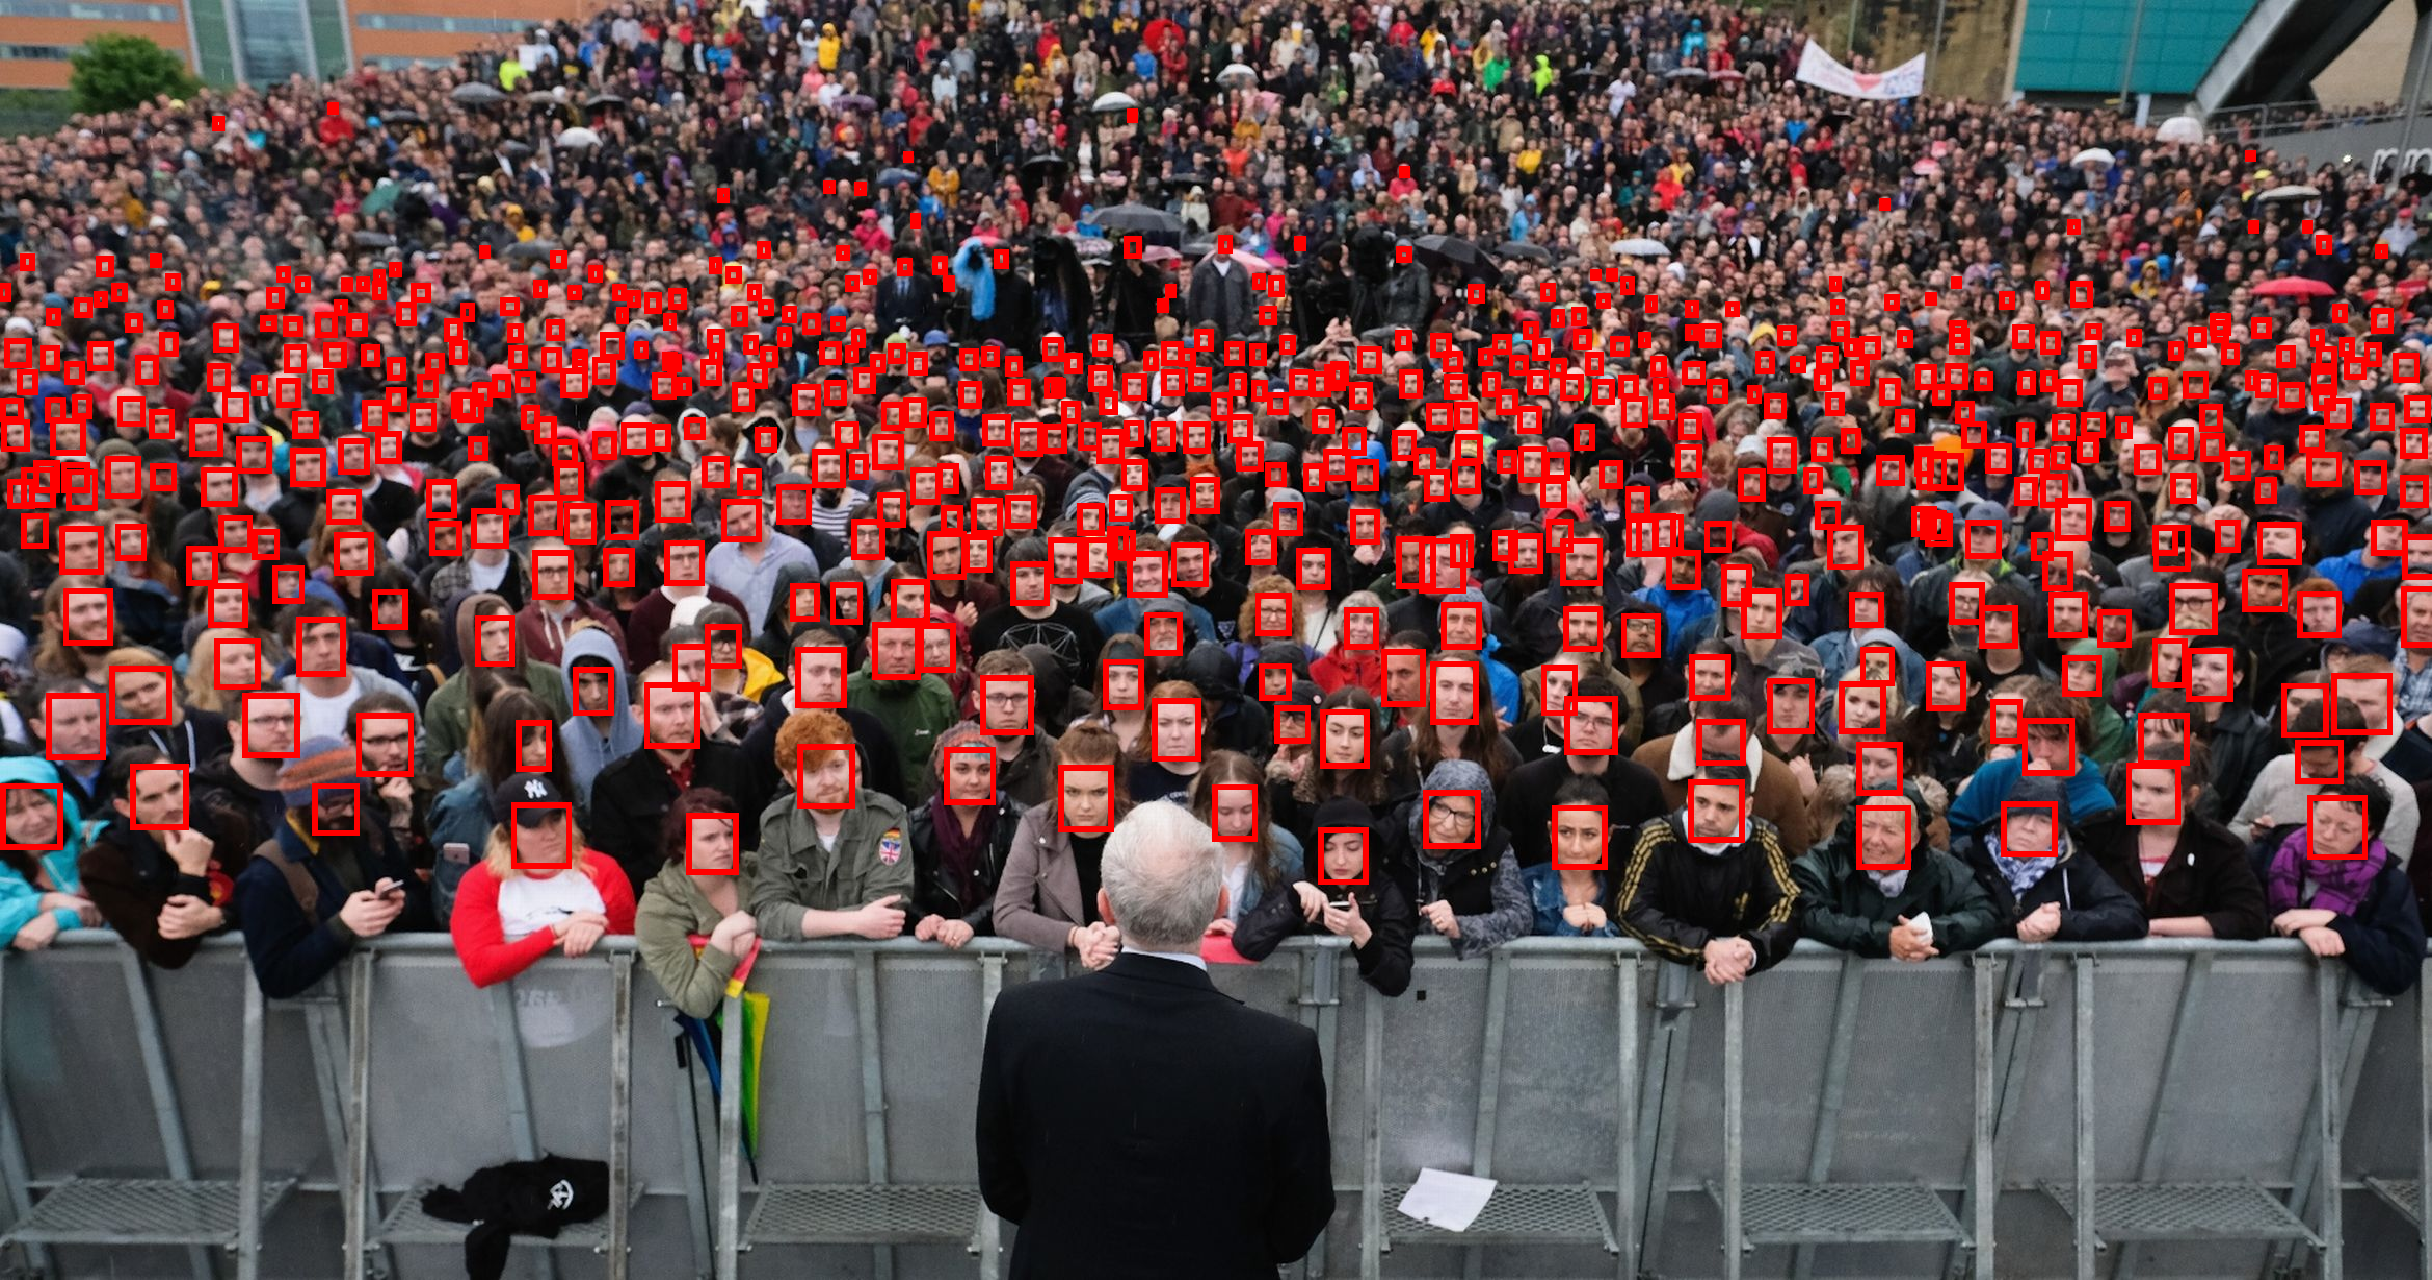
\includegraphics[scale=0.45]{resultscrowd3.png}
\end{figure}

\begin{figure}[h]
  		\includegraphics[scale=0.28]{resultscrowd4.png}
\end{figure}


%%%%%%%%%%%%%%%%%%%%%%%%%%%%%%%%%%%%%%%%%%%%%%%%%%%%%%%%%%%%%%%%%%%%%%%%%%%%%%%%%%%%
%STYLE TRANSFER
\begin{figure}
  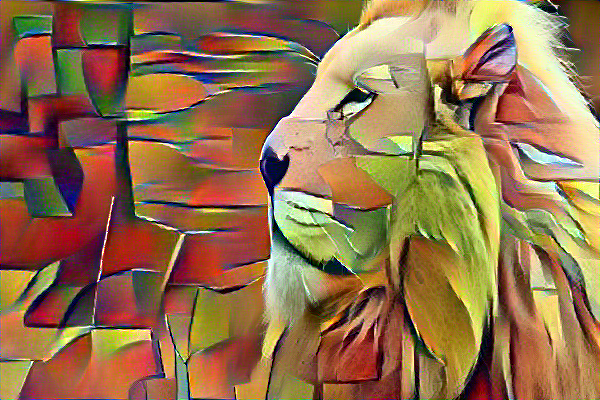
\includegraphics[scale=0.93]{lioncubism.png}
\end{figure}
\begin{figure}
  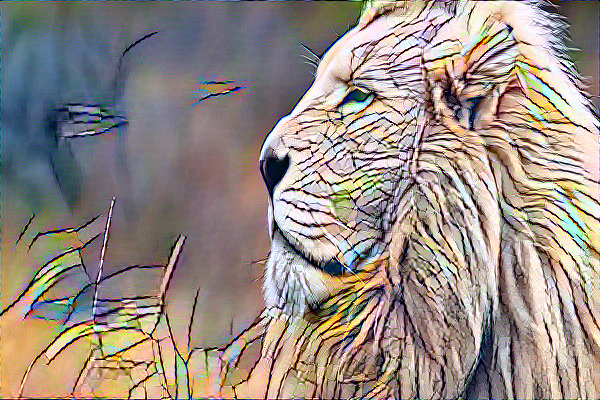
\includegraphics[scale=0.93]{lionmosaic.png}
\end{figure}
\begin{figure}
  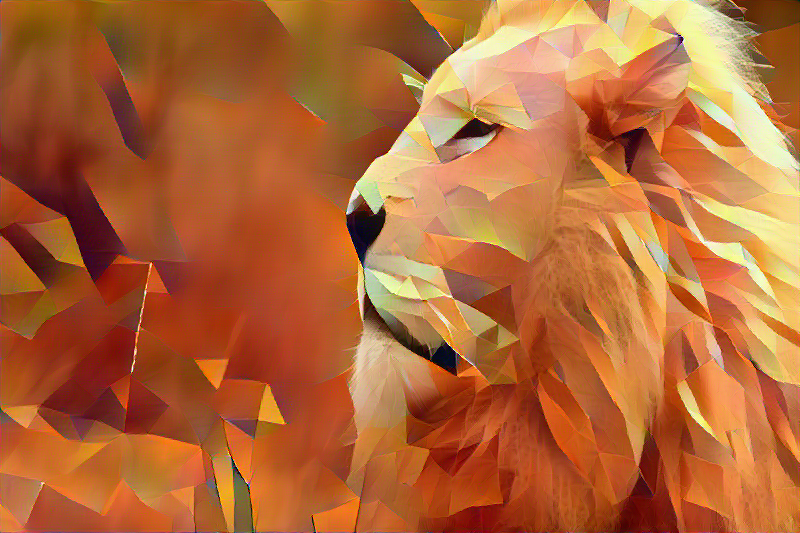
\includegraphics[scale=0.7]{lionpolyphoenix.png}
\end{figure}
\begin{figure}
  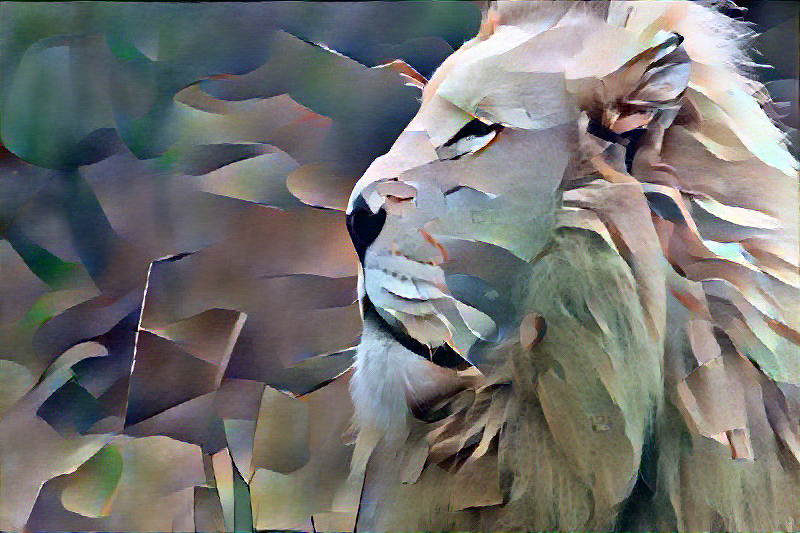
\includegraphics[scale=0.7]{lionpolyfoxstyle.png}
\end{figure}
\begin{figure}
  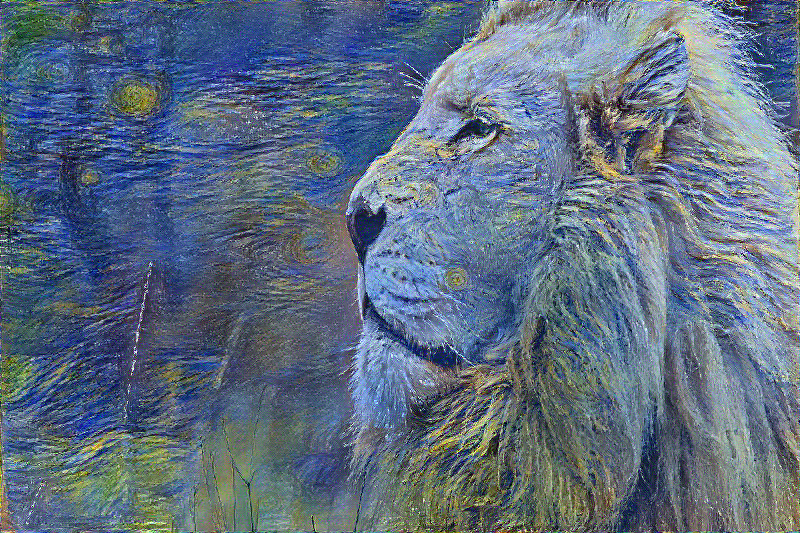
\includegraphics[scale=0.7]{lionstarrynight.png}
\end{figure}
\begin{figure}
  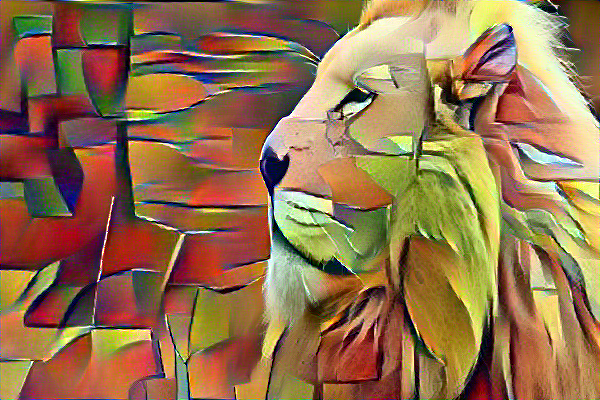
\includegraphics[scale=0.93]{lioncubism.png}
\end{figure}
\begin{figure}
  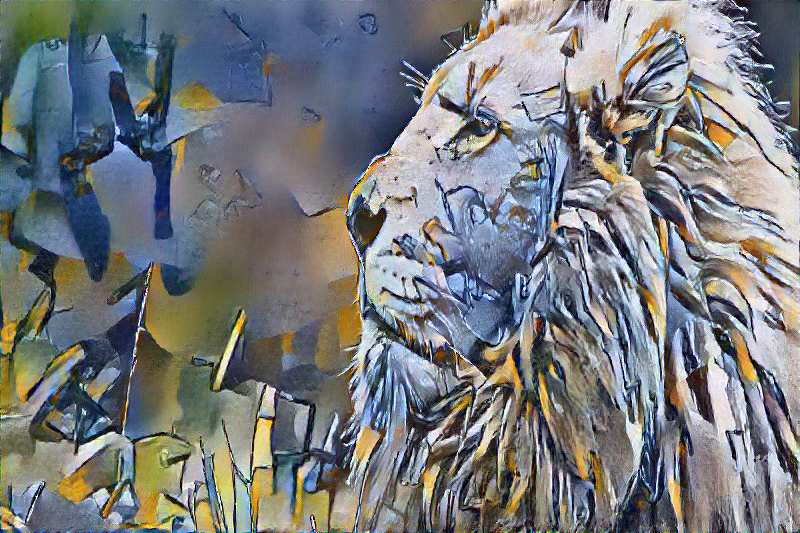
\includegraphics[scale=0.7]{lionphoenix.png}
\end{figure}
\newpage

\begin{figure}
\begin{minipage}{.5\textwidth}
    	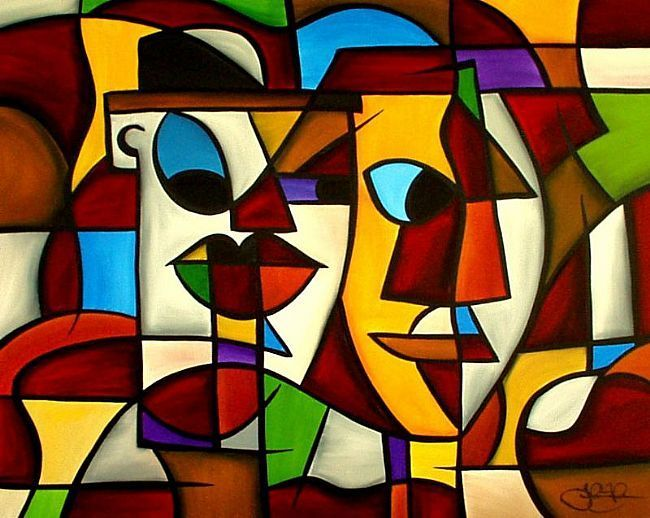
\includegraphics[scale=0.5]{happycubism.jpg}

    	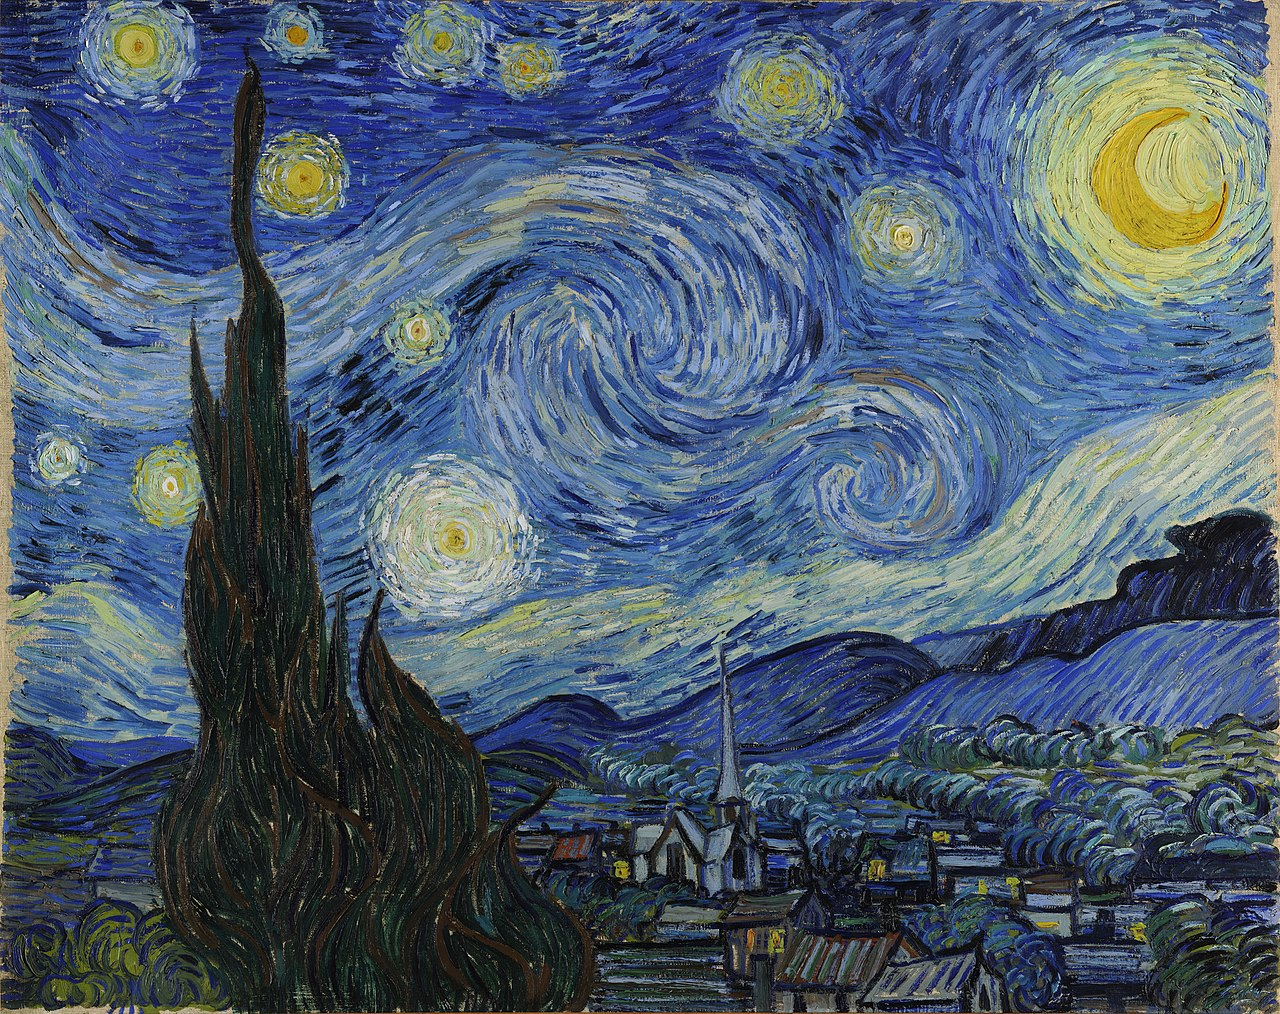
\includegraphics[scale=0.29]{starrynight.jpg}
    		
\end{minipage}%
\begin{minipage}{.5\textwidth}
  	
\includegraphics[scale=1.0]{mosaic.jpg}
  	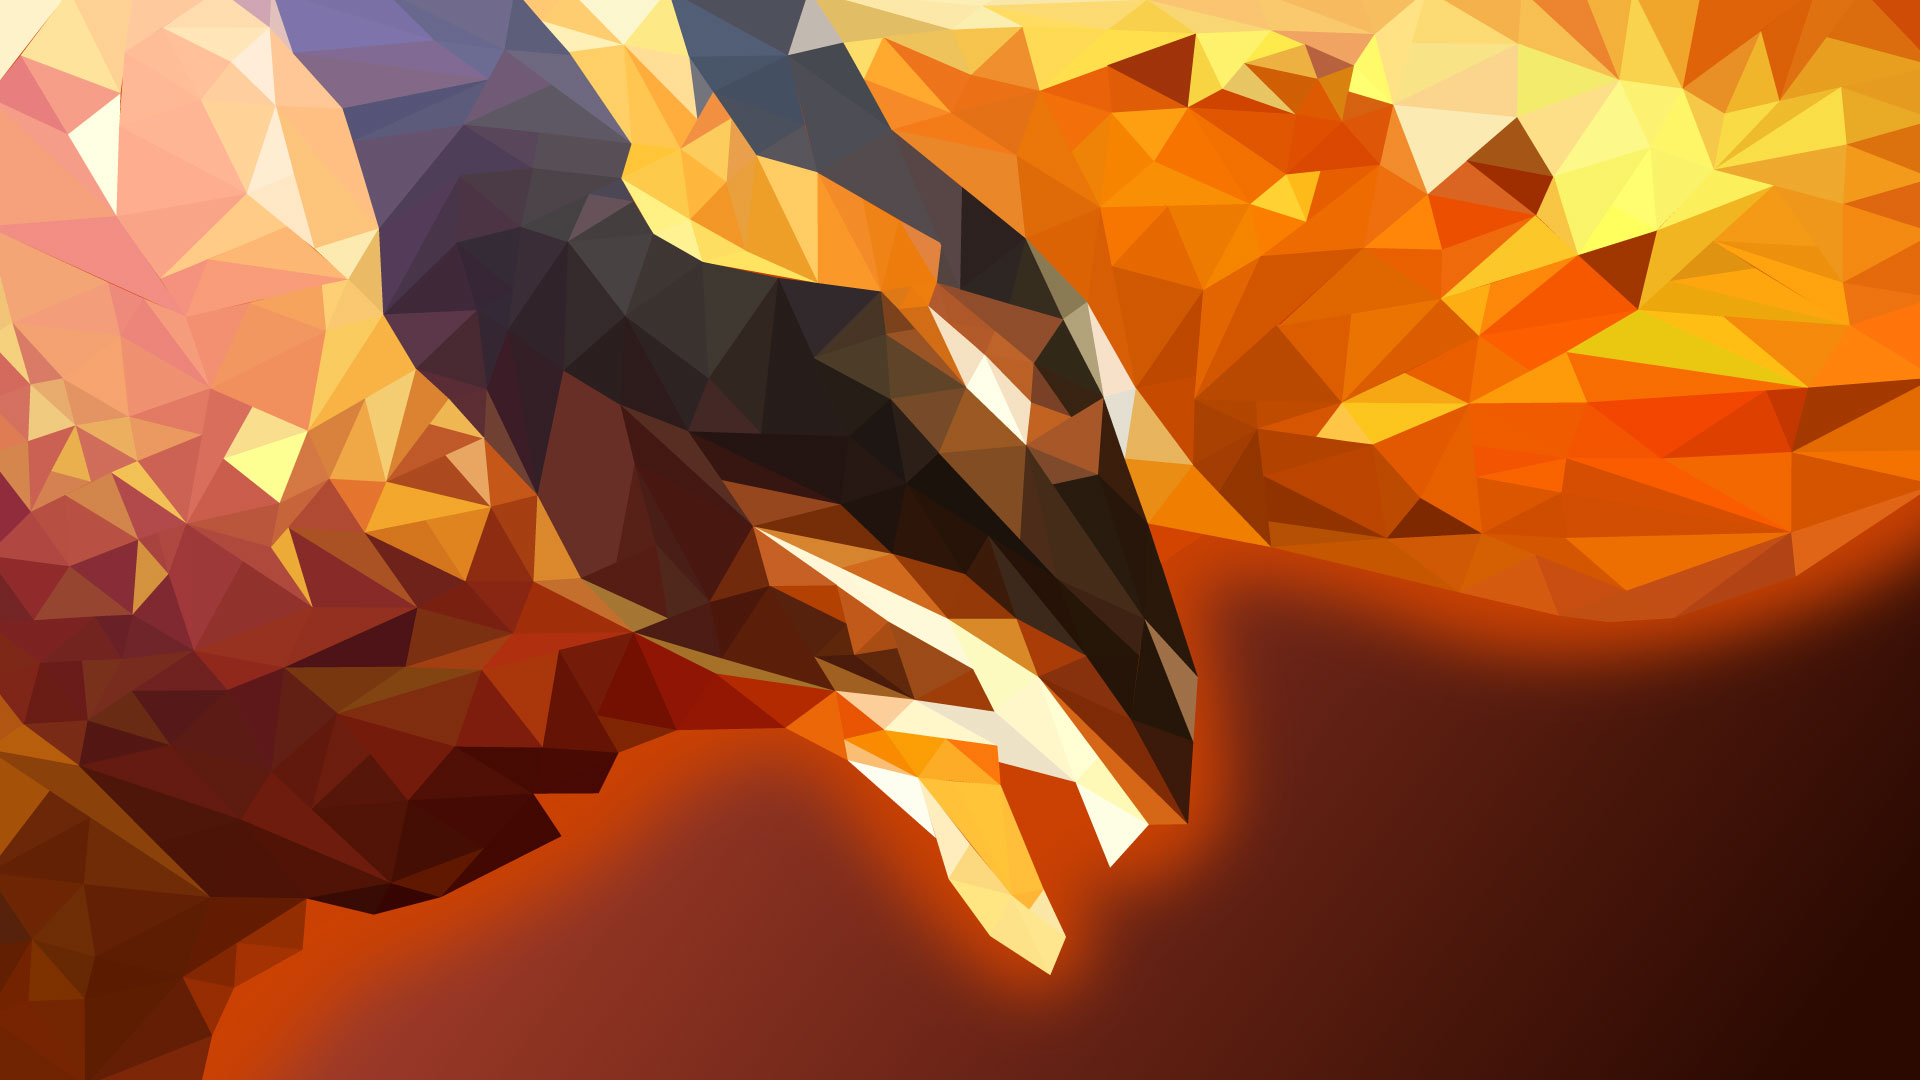
\includegraphics[scale=0.22]{polyphoenix.jpg}
\end{minipage}
\end{figure}

\begin{figure}
\begin{minipage}{.5\textwidth}
  	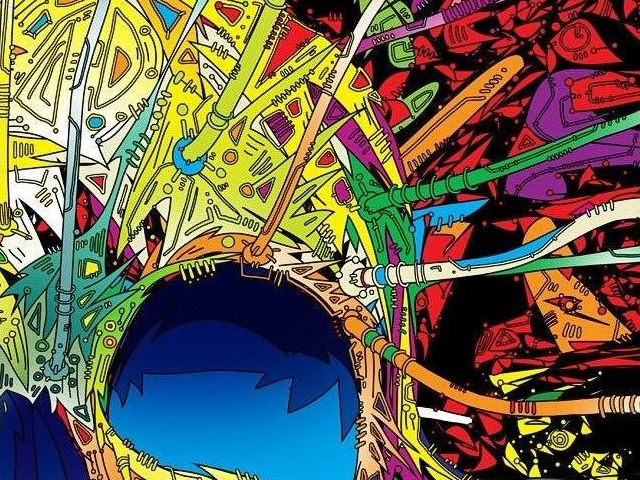
\includegraphics[scale=0.55]{acidcrop.png}
  	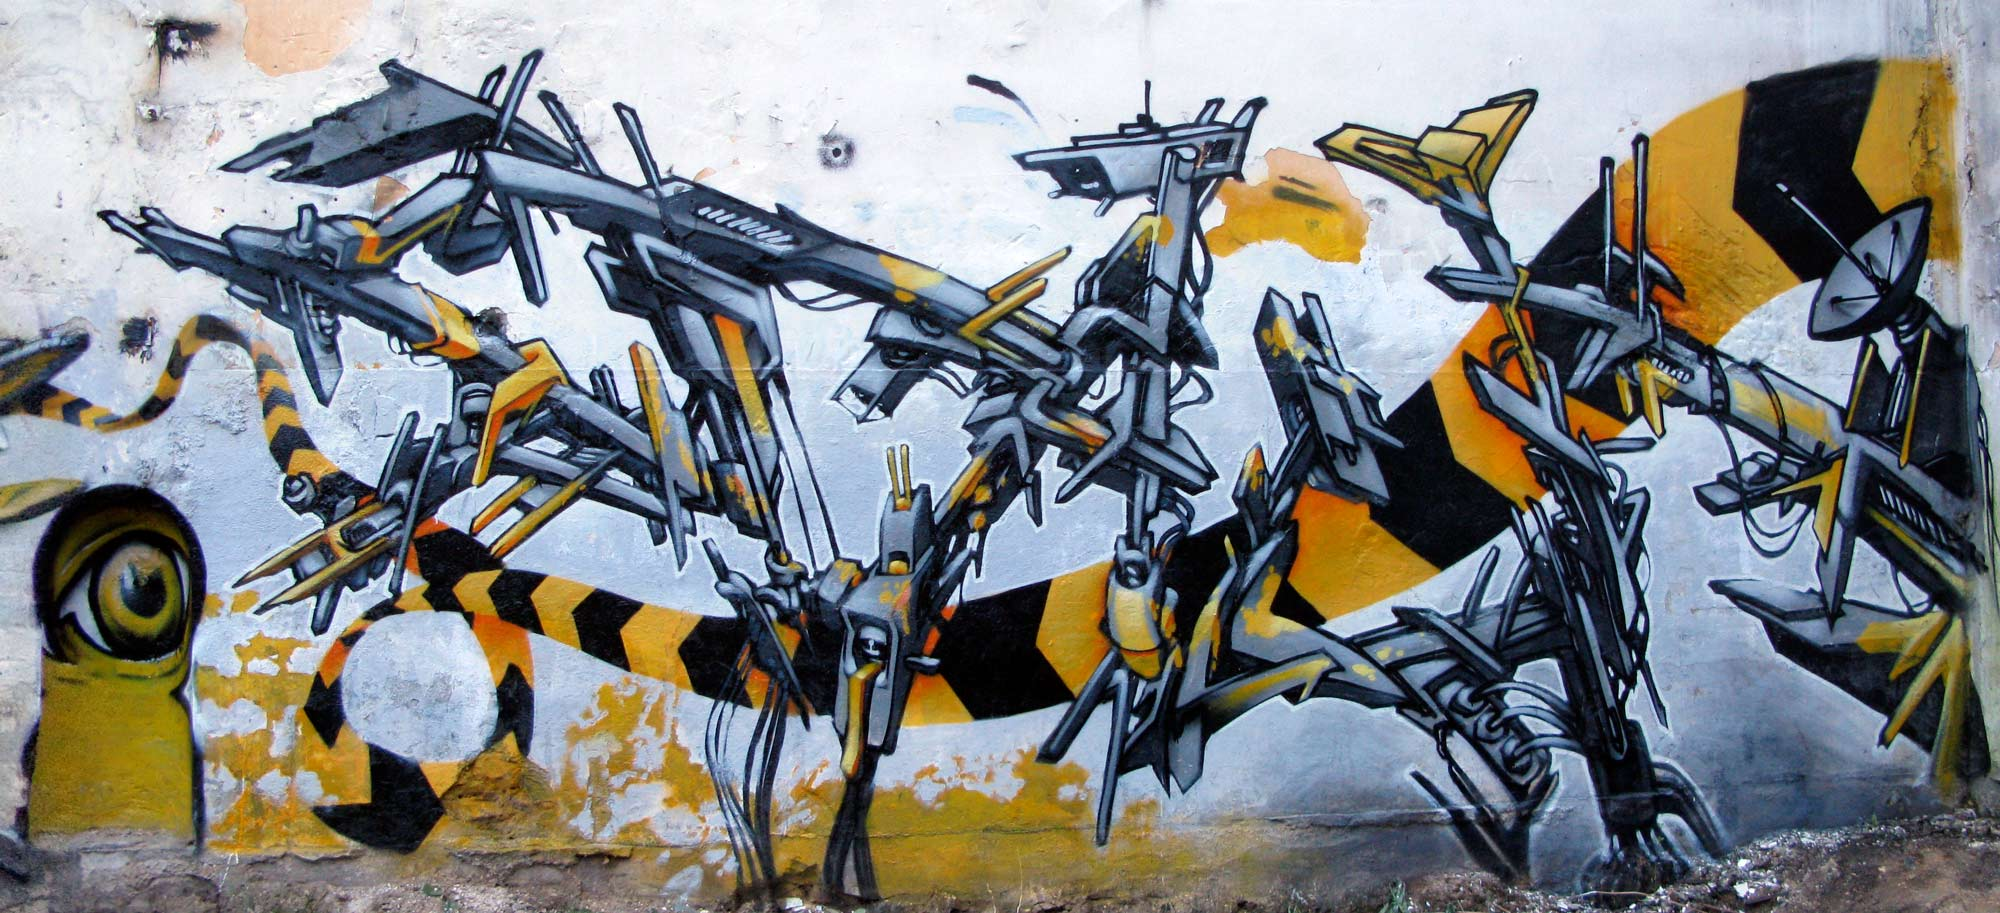
\includegraphics[scale=0.24]{graffiti.jpg}
\end{minipage}
\end{figure}

\begin{figure}
\begin{minipage}{.5\textwidth}
  	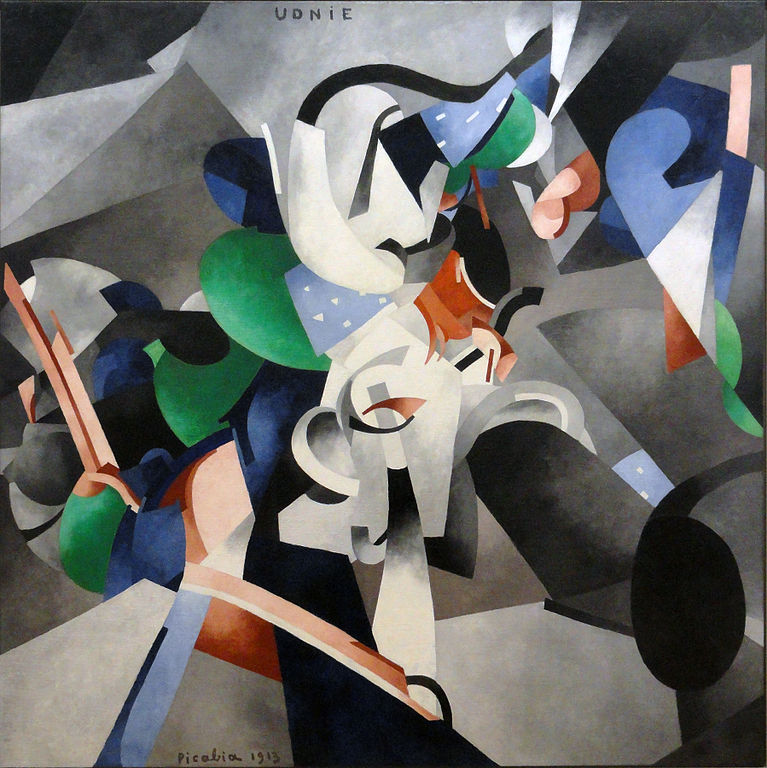
\includegraphics[scale=0.4]{polyfoxstyle.png}
  	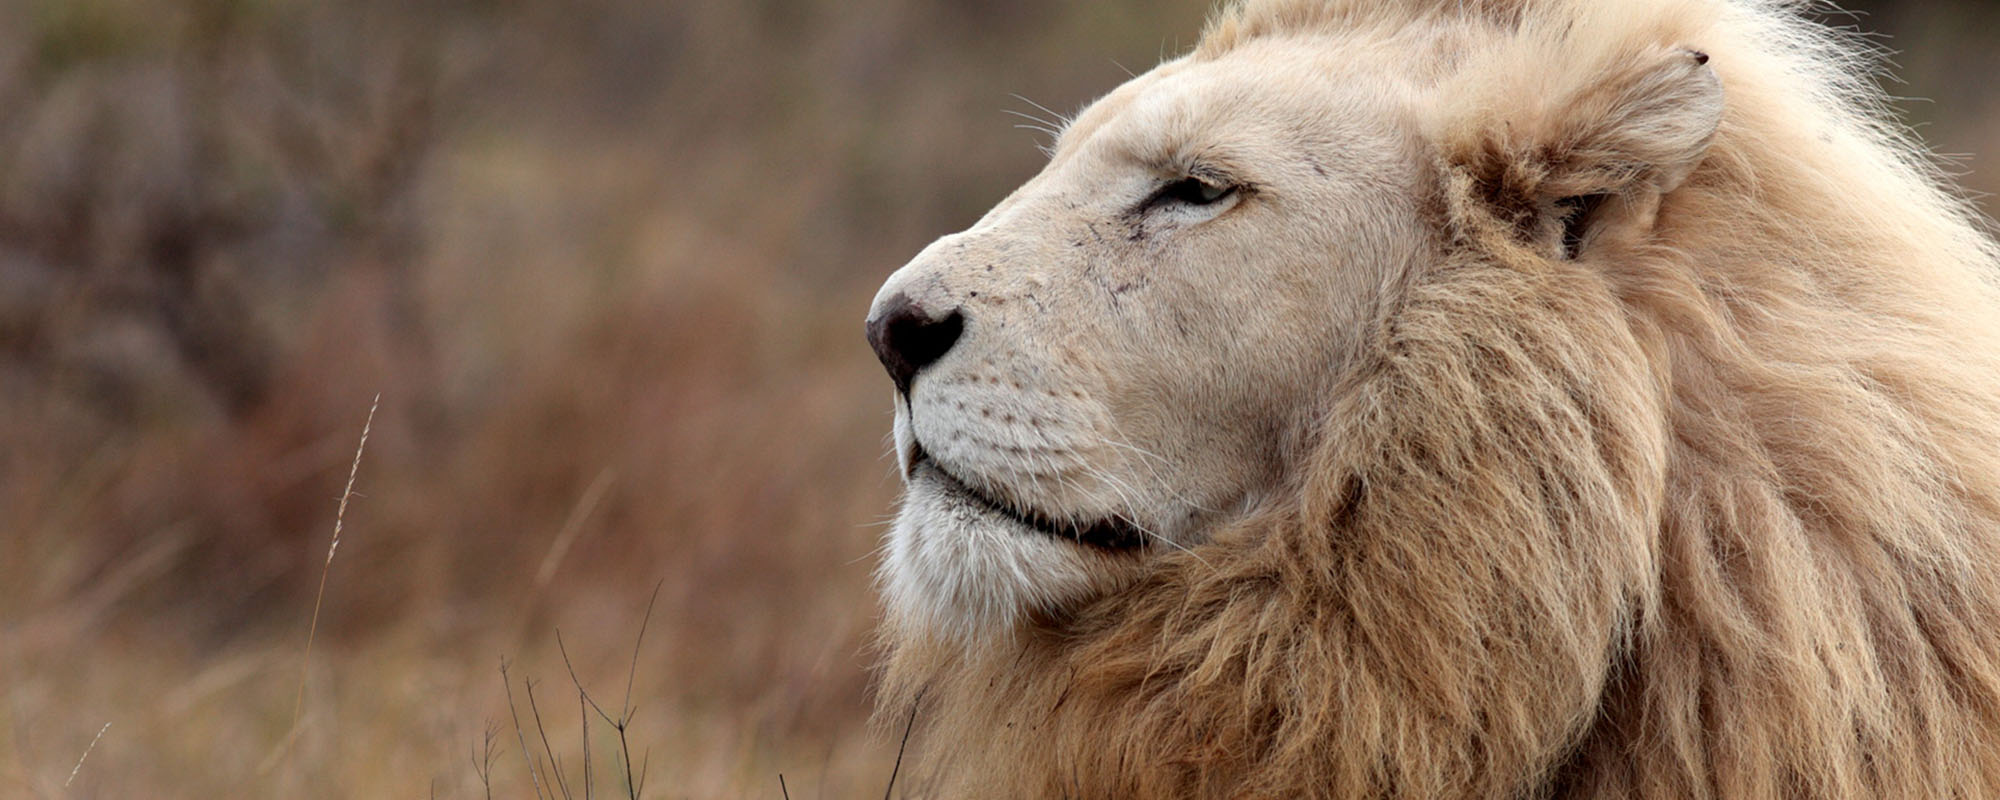
\includegraphics[scale=0.3]{lion.png}
\end{minipage}
\end{figure}



\end{document}


